\documentclass[12pt,leqno]{article}
\usepackage{bbm}
\usepackage{amsmath,amsthm,amssymb}    % need for subequations
\usepackage{paralist}
\usepackage{graphicx}   % need for figures
%\usepackage{epstopdf}  % convert eps to pdf
\usepackage{verbatim}   % useful for program listings
\usepackage{subfigure}  % use for side-by-side figures
\usepackage{hyperref}   % external documents and URLs
\usepackage{graphicx,epsfig}
%\usepackage{refcheck}
\usepackage{multirow}
\usepackage{float}
\usepackage{color}
\restylefloat{table}
\usepackage{authblk}
%\usepackage[round]{natbib}
\usepackage[numbers]{natbib}
\usepackage[toc,page]{appendix}
\usepackage{tikz}
\usetikzlibrary{shapes.geometric, arrows, positioning,automata,calc}
\tikzstyle{startstop} = [rectangle, rounded corners, minimum width=2cm, minimum height=0.75cm,text centered, draw=black]
\tikzstyle{arrow} = [thick,->,>=stealth]


%\usepackage{amssymb,amsmath,epsfig,amsfonts,epic,eepic,epsf,amsthm}
\def\R{\mathbb R}
\newcommand{\ds}{\displaystyle}
\newcommand{\J}{\mathcal{J}}
\newcommand{\K}{\mathcal{K}}
%\newcommand{\mR1}{\mathcal{R}_1}
%\newcommand{\mR2}{\mathcal{R}_2}
\newcommand{\ep}{\epsilon}
\newcommand{\vep}{\varepsilon}
%\newcommand{\nn}{$-$}
%\newcommand{\ntwo}{$-2$}
%\newcommand{\none}{$-2$}
%\newcommand{\minussign}{$-$}
\newcommand{\bfF}{\bf F}
\newcommand{\bfE}{\bf E}
\newcommand{\bfzero}{\bf 0}
\newcommand{\bfbeta}{\mbox{\boldmath$\beta$}}
\newcommand{\bfalpha}{\mbox{\boldmath$\alpha$}}
\newcommand{\bfomega}{\mbox{\boldmath$\omega$}}
\newcommand{\cbeta}{\mathcal{C}_{\mbox{\boldmath$\beta$}}}
\newcommand{\bfu}{\bf u}
\newcommand{\scriptR}{\mathcal{R}}
\newcommand{\brn}{\mathcal{R}_0}

\setlength{\textwidth}{6.7in} \setlength{\oddsidemargin}{-.20in}
\setlength{\evensidemargin}{0.10in} \setlength{\textheight}{21cm}
\setlength{\topmargin}{-.70in} \setlength{\footskip}{1.5cm}
\newcommand{\mR}{$\mathbb{R}$}
%\makeatletter
% \renewcommand{\theequation}{%
%    \thesection.\arabic{equation}}
% \@addtoreset{equation}{section}
%\makeatother

\newtheorem{Theorem}{Theorem}[section]
\newtheorem{Lemma}[Theorem]{Lemma}%[section]
\newtheorem{Proposition}[Theorem]{Proposition}%[section]
\newtheorem{Corollary}[Theorem]{Corollary}%[section]
\newtheorem{Remark}[Theorem]{Remark}%[section]
\newtheorem{Comment}[Theorem]{Comment}%[section]
\newtheorem{Example}[Theorem]{Example}%[section]

\def\bz{{\mathbf z}}
\def\bn{{\mathbf n}}
\def\bX{{\mathbf X}}
\def\bx{{\mathbf x}}
\def\bee{{\mathbf e}}
%\usepackage{appendix}
\makeatletter
 \renewcommand{\theequation}{%
    \thesection.\arabic{equation}}
 \@addtoreset{equation}{section}
\makeatother
%\date{}
\usepackage[T1]{fontenc}
\usepackage[utf8]{inputenc}
\usepackage{authblk}

\begin{document}

\section{The Model}
\subsection{Model Development}
We begin by borrowing a slightly modified equation for humans in \citep{Ruan2008}. The model is based on the Ross-Macdonald model
\citep{Anderson1992}:
\begin{equation}\label{ruan}
\dot{I_h}(t) = -r_hI_h(t) + \left(\frac{k}{N_h}\right)bS_h(t-\tau_h)I_v(t-\tau_h)\theta\,. %e^{-r_h\tau_h}\,.
\end{equation}

We assume that human population remains a constant denoted by $N_h$. In (\ref{ruan}), $I_h$, $I_v$ denote the number of humans and mosquitoes infected with dengue, respectively, $r_h$ is the recovery rate (1/day) of human from dengue so that $1/r_h$ is the duration of the disease for humans, and $k$ is the biting-rate per mosquito (number of bites/day) so that the number of bites per mosquito per human per day is $k/N_h$. Let $b$ (unitless) be the probability a mosquito bite produces an infection. Then the rate of number of exposed humans produced is $(k/N_h)bS_hI_v$. Suppose the incubation period of dengue in humans is $\tau_h$ (days), then an infected human must be exposed $\tau_h$ days ago multiplied by the probability ($\theta$) that the individual remains exposed for $\tau_h$ days (not recovered or died).  Finally, we ignore immigration and emigration since the rates are much smaller than the rest of the parameters. We ignore movement of individuals and assume homogeneous mixing meaning that each individual comes in contact with all the mosquitoes. There is no evidence that humans can transmit {\it Wolbachia}. These assumptions explain the right-hand side of (\ref{ruan}).\smallskip

Equation (\ref{ruan}) is a delay equation and delay equations are harder to study (book by Hal Smith). Some researchers introduce an exposed class to avoid studying delay equations but we do not do so here. Now $N_h = S_h + I_h + R_h$ but since we assume permanent immunity, $R_h = N_h - S_h - I_h$. Actually, there are 4 serotypes of dengue and permanent immunity is only for the same serotype. It offers cross-immunity to other serotypes but the immunity decreases over time. We also assume that $\theta = e^{-r_h \tau_h}$ (exponential). Our model for humans is therefore
\begin{eqnarray}
\dot{S}_h(t) &=& \mu_hN_h - \left(\frac{k b}{N_h}\right) S_h(t-\tau_h)  I_v(t-\tau_h)e^{-r_h\tau_h} - \mu_h S_h\nonumber\\
\dot{I_h}(t) &=& -r_hI_h(t) + \left(\frac{k b}{N_h}\right)S_h(t-\tau_h)I_v(t-\tau_h)e^{-r_h\tau_h} - \mu_h I_h\label{human}
%\dot{R}_h(t) &=& r_h I_h(t)\quad \text{(not needed)}\nonumber
\end{eqnarray}
We also only model one serotype of dengue. For delay equations, it is customary to include time in delay equations; hence, $S_h(t)$ instead of $S_h$ etc. in the above equations.\smallskip 

We now turn to model mosquitoes. First we ignore {\it Wolbachia}. Incubation period for dengue is $\tau_v$, death-rate is $\mu_v$. Since life-span of mosquitoes is a few weeks, say $\mu_v = 1/(7\times 4)$, so incubation time cannot be ignored in the model. We assume that dengue does not affect birth-rate or death-rate of mosquitoes (reference needed) and there is no recovery for mosquitoes from dengue (this is true). $c$ is the probability of transmission from infected human to susceptible mosquito during a bite. We also assume that dengue cannot be transmitted to offsprings by an infected mosquito (possible but rare). For now, we don't take aquatic stage (egg, larva, pupa) into account. Then our model for mosquitoes is
\begin{eqnarray}\label{dengue}
\dot{S}_v(t) &=& \textit{birth-rate A} - \left(\frac{k c}{N_h}\right) S_v(t-\tau_v)I_h(t-\tau_v)e^{-\mu_v\tau_v} - \mu_v S_v(t)\nonumber\\
\dot{I_v}(t) &=& \left(\frac{k c}{N_h}\right)S_v(t-\tau_v)I_h(t-\tau_v)e^{-\mu_v\tau_v} - \mu_v I_v(t)\nonumber
\end{eqnarray} 

Now let us see how (\ref{dengue}) has to be changed to include {\it Wolbachia} in our model. Each one of our assumptions below need to be checked in the literature.  
\begin{enumerate}
\item\,\,Let us consider co-infection. It is clear that co-infection can only happen through birth since {\it Wolbachia} can be transmitted only through birth, and not between adult mosquitoes or by biting an {\it Wolbachia}-infected human. A female mosquito lay eggs which are fertilized by {\it Wolbachia}-infected male, then a large percentage of the eggs do not hatch (this is called cytoplasmic incompatiblity, CI). We assume 100\% do not hatch in our model. A {\it Wolbachia}-infected female mosquito lay eggs fertilized by a dengue-infected male mosquito, then eggs may be co-infected. We assume that this does not happen. So no co-infection. This simplifies the model by Hughes and Britton. 
\item\,\,{\it Wolbachia} can only be transmitted through birth maternally and unlike dengue there is no incubation period.
\item\,\,We study only one strain of {\it Wolbachia} even though there are 4 strains. Parameters are strain-dependent. There is one vaccine for dengue but it is not commonly given to adults.  The chance of developing dengue hemorrhagic fever is small for adults. Most of the time, adults just develop some flu-like symtoms and recover.
\item\,\,We only model female mosquitoes because only female mosquitoes bite. We also assume that male and female mosquitoes are equal in number.
\item\,\,Cytoplasmic Incompatibiltiyh (CI) means that an infected male and an uninfected female give rise to eggs that only certain percentage, $1-s_h$, of the eggs hatches. $s_h$ is {\it Wolbachia} strain dependent. We shall later assume $s_h = 1.$
\item\,\,{\it Wolbachia} infected mosquitoes also have lower birth-rate and higher death-rate.  
\item\,\, Equation for {\it Wolbachia}-infected moquitoes, $I_w$, is
\begin{equation}\label{Wolbachia}
\dot{I}(t) = \textit{birth-rate B} - \mu_w I_w\,. 
\end{equation}
\item\,\,
We {\it Wolbachia}-infected mosquitoes have shorter life-span: $\mu_w > \mu_v$. We also assume density dependent per-capita growth rate $f$ (all mosquitoes). When temperature is warm and that are plenty of rainfall, then eggs hatches in one or two days. The time from eggs to emerge as an adult mosquito is about 10-14 days (ideal case).
So birth-rate B  should just be $f(S_v+I_v+I_w)(1-s_f)b_z v I_w$, where $b_z$ is the birth-rate of wild-type mosquitoes. We assume success of maternal transmission of {\it Wolbachia} is the fraction $v$.
\end{enumerate}  

Let us model birth-rate A.  I borrow this idea from \cite{Hughes2013}, the paragraph right under Table 1 p. 801. Ignore the life-cycle of mosquitoes for the moment. Let $N_{z} = S_v+I_v+I_w$, total number of mosquitoes. The number of offsprings is $b_z(S_v + I_v) + (1-v)b_z(1-s_f)I_w)$, where $v$ is fraction of offsprings from {\it Wolbachia}-infected female that are also {\it Wolbachia}-infected. But not all eggs are going to hatch because of CI. Assume rBelow andom mating, the probability of inviability is $s_hI_w/(S_v+I_v+I_w)$, where $s_h$ is the probability of {\it Wolbachia}-infected male, {\it Wolbachia}-uninfected female produce inviable eggs. Therefore, 
\[
\textit{birth-rate A} = f(N_z)(1 - s_h I_w/N_z)b_z(S_v+I_v+(1-v)(1-s_f)I_w)\,.
\]
We assume that male and female mosquitoes are equal in number. See p. 799 of \citep{Hughes2013} second assumption. For simplicity, we assume that $v=1$ and $s_h=1$. So maternal transmission of {\it Wolbachia} is 100\% successful and CI is also 100\%.\smallskip

To incorporate life-cycle into our model, let $\tau_d$ be the number of days from laying eggs to emerge as adult mosquitoes. This number is around 10days under ideal situations but varies widely depending on abundance supply of water and food. So birth-rate terms have to be delayed by $\tau_d$ days. 

\begin{tikzpicture}[node distance=2.5cm and 1.5cm, align=center] 
 
\node (Ih) [startstop] at (0,0) {$I_h$};
\node (Iv) [startstop] at (5,0) {$I_v$};
\node (Sh) [startstop] at (0,-4) {$S_h$};
\node (Sv) [startstop] at (5,-4){$S_v$};
\node (Iw) [startstop] at (10,-2) {$I_w$};





\draw[<-] (-3,0) -- ( $ (-3,0)!.67!(0,0) $ ) node [midway, sloped, above] {$\mu_hI_h-vI_h$};
\draw[<-] (-3,-4) -- ( $ (-3,-4)!.67!(0,-4) $ ) node [midway, sloped, above] {$\mu_hS_h$};
\draw[->] (0,-6) -- ( $ (0,-6)!.75!(0,-4) $ ) node [midway, sloped, above] {$\mu_hN_h$};
\draw[->] (5,-6) -- ( $ (5,-6)!.75!(5,-4) $ ) node [midway, sloped, above] {$Birth_A$};
\draw[->] (6,-4) -- ( $ (6,-4)!.67!(9,-4) $ ) node [midway, sloped, above] {$\mu_vS_v$};
\draw[->] (5,0.35) -- ( $ (5,0.35)!.75!(5,2.35) $ ) node [midway, sloped, above] {$\mu_vI_v$};
\draw[->] (11,-1.65) -- ( $ (11,-1.65)!.75!(14,-0.35) $ ) node [midway, sloped, above] {$\mu_wI_w$};
\draw [->] (Iw) to[out=-80, in=-90] (12,-2)    to[out=90,in=80](Iw) ;

\draw [arrow] (Sh) --  node[above,sloped]{Infection}(Ih);
\draw [arrow] (Sv) --  node[below,sloped]{Infection}(Iv);
\draw [arrow] (Ih) -- (Sv);
\draw [arrow] (Iv) -- (Sh);
\draw [arrow] (Iv) -- (Iw);
\draw [arrow] (Sv) -- node[above,sloped]{$Birth_B$}(Iw) ;
%\draw [arrow] (second) -- node[xshift=-0.12cm] {Mixture model} (third);
%\draw [arrow] (third) -- node[xshift=-0.10cm] {Individual p-values} (fourth);
\end{tikzpicture}

The full model is
\begin{eqnarray}\label{model}
\dot{S}_h(t) &=&  \mu_hN_h - \left(\frac{k b}{N_h}\right) S_h(t-\tau_h)  I_v(t-\tau_h)e^{-\gamma\tau_h} - \mu_hS_h\nonumber\\
\dot{I}_h(t) &=& -\gamma I_h(t) + \left(\frac{k b}{N_h}\right)S_h(t-\tau_h)I_v(t-\tau_h)e^{-\gamma\tau_h} - \mu_h I_h\nonumber\\
\dot{S}_v(t) &=& \Big[f(N_z)\left(1 - \frac{I_w}{N_z}\right)(S_v+I_v)\Big](t-\tau_d)\nonumber \\
& & - \left(\frac{k c}{N_h}\right) S_v(t-\tau_v)I_h(t-\tau_v)e^{-\mu_v\tau_v} - \mu_v S_v(t)\label{modelux}\\\nonumber \\
\dot{I}_v(t) &=& \left(\frac{k c}{N_h}\right)S_v(t-\tau_v)I_h(t-\tau_v)e^{-\mu_v\tau_v} - \mu_v I_v(t)\nonumber\\
\dot{I}_w(t) &=& \big[f(N_z)(1-s_f)I_w\big](t-\tau_d) - \mu_w I_w\nonumber\,. 
\end{eqnarray} 
Here, $N_z = S_v + I_v + I_w$ and we assume that 
$f(N) = \max\left\{b_0\left(1-\displaystyle\frac{N}{K}\right)+\displaystyle\frac{\mu_v N}{K},0\right\}$. In \citep{Hughes2013}, $f(N) = b_0e^{-hN^{\alpha}}$. The model has $12$ positive parameters. Their estimated values found in the literature are given in Table~\ref{TableParameters}.\smallskip


\begin{table}[!ht]
%\begin{adjustwidth}{-0.75in}{0in}
\caption{{\bf Parameter Values.} \,Values taken from Table 3 of \citep{Manore2014}. We chose
the values for \textit{Ae. aegypti} in \citep{Manore2014} although \textit{Ae. albopictus} is also a
possible carrier. Values of IIP and EIP are taken from the Internet. Also available in
\citep{Chan2012} but they don't seem to have an agreed number. {\color{red} This table needs to be updated}} 
    %\begin{tabular}{ | l | l | l | p{7cm} |}
    \begin{tabular}{ l * {3}{l}}
    \hline
    Parameter (unit) & Range &Meaning \\ \hline
    $b$ & $(0.10,0.75)$ & Probability of infection from infected mosquito to susceptible human \\ \hline
    $c$ & $(0.10,0.75)$ & Probability of infection from infected human to susceptible mosquito \\ \hline
    $k$ & $(0.33,1)$ & Biting rate \\ \hline
    $K/N_h$ & \{1,2,...,n\} & Ratio of mosquito to human population size\\ \hline
    $\mu_h$\,\,(1/years) & $(1/76,1/60)$ & Human death-rate \\ \hline
    $\mu_v$\,\,(1/days) & $(1/42,1/8)$ & Mosquito death-rate \\ \hline
		$\mu_w$\,\,(1/days) & check & Death-rate of \textit{\it Wolbachia}-infected mosquitoes \\ \hline
    $\gamma$\,\,(1/days) & $(1/12,1/4)$ & Human recovery rate \\ \hline
    $\tau_h$\,\,(days) & $(4,10)$  &IIP for humans \\ \hline
    $\tau_v$\,\,(days) & $(4,10)$  &EIP for mosquitoes at $30^o$C \\ \hline
		$\tau_d$\,\,(days) & $(10,14)$  & Development from eggs to eclosion under ideal situation.\\ \hline		
    $b_0$\,\,(1/days) & $(\mu_v,\mu_w/(1-s_f))$  & Birth-rate of wildtype mosquitoes\\ \hline
    %$s_h$ & $(s_h^*,1)$ & Reduction in birth-rate due to CI \\ \hline
    %$a$\,\, & $(0.01,0.10)$  & Rate of release in fraction of $K$ \\ \hline
    %$L_{period}$\,\,(days) & $\{1,...,7\}$  & Duration of each release \\ \hline
    %$d$\,\,(days) & $\{1,...,30\}$  & Time between two releases \\ \hline
    %$M$  & $\{1,...,10\}$  & Number of releases \\ \hline
    \end{tabular}
\begin{flushleft} 
\end{flushleft}
\label{TableParameters}
%\end{adjustwidth}
\end{table}



To analyze the limiting (as time goes to infinity) behavior of the solutions of the above model, we first find its steady-states, which are constant solutions of (\ref{models}). There are five steady-states: $E_1, E_2, E_3, E_4, E_5$. To define them, we introduce some notations. Let
\begin{eqnarray*}
\beta_1 &=& \frac{kb}{N_h}e^{-\gamma\tau_h}\,,\;\;\beta_2 = \frac{kc}{N_h}e^{-\mu_v\tau_v}\\
J &:=& b_0(1-s_f) - \mu_w\\
%J1 &:=& (b_0(1-s_f)-\mu_w)/(b_0-\mu_v)\quad(new)\\
A_1 &:=& \mu_h\beta_2N_h + (\gamma + \mu_h)\mu_v\\
A_2 &:=& \mu_h(\beta_1\beta_2 KN_h - (\gamma +\mu_h)\mu_v)\\
%&=& (\gamma + \mu_h)\mu_h\mu_v\,(\brn -1)\\
A_3 %&:=& b_0\beta_1\mu_v(1-s_f) + b_0\mu_h\mu_w - \beta_1\mu_v\mu_w - \mu_h\mu_v\mu_w\\
&:=& \beta_1\mu_vKJ + (b_0-\mu_v)\mu_h\mu_w\\
%&=& \beta_1\mu_v(b_0-\mu_v)(J-\mu_h\mu_w)\quad(new)\\
%A_4 &=& b_0\beta_1\beta_2(1-s_f)- b_0\gamma\mu_w -b_0\mu_h\mu_w - \beta_1\beta_2\mu_w + \gamma\mu_v\mu_w+\,\mu_h\mu_v\mu_w \\
A_4 %&:=& \beta_1\beta_2(b_0(1-s_f)-\mu_w) - (\gamma+\mu_h)(b_0 - \mu_v)\mu_w\\
%A_4 &=& \beta_1\beta_2(b_0(1-s_f) - \mu_w) - \mu_w(b_0-\mu_v)(\gamma+\mu_h)\\
&:=& \beta_1\beta_2 KN_h J - (b_0-\mu_v)(\gamma+\mu_h)\mu_w\\
%&=& (b_0-\mu_v)\,(J\beta_1\beta_2 - (\gamma+\mu_h)\mu_w)\quad (new)
%A_5 &=& \beta_1\mu_w(b_0-\mu_v)(\mu_h\beta_2+\gamma\mu_v+\mu_h\mu_v)
%W_0 &:=& \frac{(\mu_w-\mu_v(1-s_f))J}{(1-s_f)(b_0-\mu_v)\mu_w}
\end{eqnarray*}
Then, the steady states are:
\begin{eqnarray*}
E_1 &:=& (N_h,0,K,0,0)\\
E_2 &:=& \left(N_h,0,0,0,\frac{KJ}{(1-s_f)(b_0-\mu_v)}\right)\\
%&=& \left(1,0,0,0,\frac{J}{1-s_f}\right)\quad (new)\\
E_3 &:=& \left(N_h,0,\frac{\mu_v KJ}{(b_0-\mu_v)\mu_w},0,
\frac{(\mu_w-\mu_v(1-s_f))KJ}{(1-s_f)(b_0-\mu_v)\mu_w}\right)\\
%&=& \left(1,0,\frac{\mu_v J}{\mu_w},0,\frac{(\mu_w-\mu_v(1-s_f))J}{(1-s_f)\mu_w}\right)\quad (new)\\
E_4 &:=& \left(\frac{A_1}{\beta_2(\beta_1K+\mu_h)},\frac{A_2}{\beta_2(\beta_1K+\mu_h)(\gamma+\mu_h)},
\frac{\mu_v(\beta_1K+\mu_h)(\gamma+\mu_h)}{A_1\beta_1},\frac{A_2}{A_1\beta_1},0\right)\\
%&=& \left(A_1^*,\frac{A_2^*}{\gamma+\mu_h},
%\frac{\mu_v(\gamma+\mu_h)}{A_1^*\beta_1\beta_2},\frac{A_2^*}{A_1^*\beta_1},0\right)\quad (new)\\
E_5 &:=& \left(\frac{\mu_w(b_0-\mu_v)A_1}{A_3\beta_2},\frac{\mu_h\mu_vA_4}{\beta_2(\gamma+\mu_h)A_3},\frac{\mu_v(\gamma+\mu_h)A_3}{\beta_1\mu_w(b_0-\mu_v)A_1},\frac{\mu_h\mu_vA_4}{\beta_1\mu_w(b_0-\mu_v)A_1},\right.\\
& &\;\;\left.\,\frac{(\mu_w-\mu_v(1-s_f))KJ}{(1-s_f)(b_0-\mu_v)\mu_w}\right)\\
\end{eqnarray*}

The traditional ways to control mosquitoes are to remove standing water and spray insecticides. These methods reduce $b_0$ in the model. However, we always assume that\smallskip

(H1)$\;\;b_0 > \mu_v$.\smallskip

\noindent Since mosquitoes infected with {\it Wolbachia} have higher death rates than those uninfected, we also assume throughout the paper that \smallskip

(H2)$\;\;\mu_w > \mu_v$.\smallskip

\noindent Note that if $J>0$, then (H2) implies (H1). According to \citep[display (2)]{Ruan2008}, the Basic Reproduction number for the above model is
$$
\brn := \displaystyle\frac{\beta_1\beta_2KN_h}{(\gamma+\mu_h)\mu_v} = \left(\displaystyle\frac{k^2bcK }{N_h(\gamma+\mu_h)\mu_v}\right)e^{-\gamma\tau_h} e^{-\mu_v\tau_v}.
$$
\begin{Proposition}\label{totaldengue}
(i) The total number of mosquitoes for $E_1$ and $E_4$ are both equals to $K$. The total number of mosquitoes for $E_2, E_3$ and $E_5$ are the same and equals to $KJ/((1-s_f)(b_0-\mu_v))$; (ii) $E_1$ always exists and $E_4$ exists if and only if $\mathcal{R}_0>1$; (iii) If $J < 0$, then $E_2, E_3$ and $E_5$ do not exist; (iv) If $J > 0$, then $E_2, E_3$ exist and $E_5$ exists if and only if 
\begin{equation}\label{A4pos}
%\beta_1\beta_2[b_0(1-s_f)-\mu_w] > (\gamma + \mu_h)(b_0-\mu_v)\mu_w\\%
\mathcal{R}_0 > r^* := \displaystyle\frac{(b_0-\mu_v)\mu_w}{\mu_vJ} > 1.
\end{equation}
\end{Proposition}

We now investigate the long term behavior of solutions to (\ref{model}). There are two types of behavior. First is convergence to a steady-state and second is sustained oscillation. They have implications to the actual behavior of the dengue virus and whether our strategy of releasing {\it Wolbachia} into the mosquito population is effective or not. For example, we shall show later that $E_2$ and $E_4$ if exist are both locally asymptotically stable but $E_2$ is desirable and $E_4$ is not. If solutions converge to $E_2$, then eventually all mosquitoes carry {\it Wolbachia} so the strategy succeeded but if solutions converge to $E_4$, then the opposite occurs; no mosquito is infected with {\it Wolbachia} and the strategy failed.\smallskip

A steady-state solution $E$ is said to be locally asymptotically stable (l.a.s.) if there exists a neighborhood in the state space containing $E$ in its interior such that if $S_h,I_h,S_v,I_v,I_w$ start from this neighborhood at time zero, then $S_h(t),I_h(t),S_v(t),I_v(t),I_w(t)$ converge to $E$ as time goes to infinity. If solutions to (\ref{model}) exhibit sustained oscillations, that means there are periodic outbreak of the disease that won't go away with time. These sustained oscillations (stable periodic solution) often bifurcate from a steady-state, which becomes unstable as certain parameter crosses a critical value. The proofs of the following propositions may be found in the Appendix.\smallskip

For stability analysis, in addition to (H1) and (H2), we will also assume that\smallskip

(H3) $\;\;b_0 < 3\mu_v.$\smallskip

(H4) $\;\;\mu_v\tau_h < 1$. This is biologically reasonable.\smallskip

\begin{Proposition}\label{E1E4stable}
Let $\mathcal{R}_0 < 1$. Then $E_1$ is stable and $E_4$ does not exist. If $\mathcal{R}_0 > 1$, then $E_1$ becomes unstable, $E_4$ exists and is l.a.s. for sufficiently small $\mu_h > 0$.
\end{Proposition}

\begin{Proposition}\label{E2stable}
Let $J > 0$. Then $E_2$ exists and is l.a.s.
\end{Proposition}

The analysis of $E_3$ and $E_5$ are more complicated. Their characteristic equations share a common factor of the form
$H(\lambda) = a_2 (e^{-\lambda \tau_d})^2 + a_1(\lambda) e^{-\lambda\tau_d} + a_0(\lambda).$ Here, $a_2$ is a constant independent of the delays, $a_1$ is linear in $\lambda$ with coefficients independent of the delays, and $a_0(\lambda) = \mu_w^2(\lambda + \mu_v)(\lambda + \mu_w)$. The equation $H(\lambda)=0$ in general has positive root, which renders both $E_3$ and $E_5$ unstable.

\begin{Proposition}\label{E3E5unstable}
Let $J > 0$. Then aside from the instability resulting from the positive roots of $H(\lambda)=0$, $E_3$ is stable if $\mathcal{R}_0 < r^*$ and unstable if $\mathcal{R}_0 > r^*$. $E_5$ does not exist if $\mathcal{R}_0 < r^*$ and aside from the instability resulting from the positive roots of $H(\lambda)=0$, it is l.a.s. for sufficiently small $\mu_h > 0$.
\end{Proposition}

{\color{red} We need to consider the case when $b_0$ is very large.}

\section{Appendix}\label{append}
In this Appendix, we use the same notations as in the main body of the text but their meanings are slightly different.\smallskip

We non-dimensionalize (\ref{model}) by dividing the first two equations of (\ref{model}) by $N_h$ and the last three equations by $K$. Let $\beta_1 = (kbK/N_h)e^{-\gamma\tau_h}$ and let $\beta_2 = kce^{-\mu_v\tau_v}$. Then (\ref{model}) becomes
\begin{eqnarray}\label{models}
\dot{S}_h(t) &=&  \mu_h - \beta_1 S_h(t-\tau_h)  I_v(t-\tau_h) - \mu_hS_h\nonumber\\
\dot{I}_h(t) &=& -\gamma I_h(t) + \beta_1 S_h(t-\tau_h)I_v(t-\tau_h) - \mu_h I_h\nonumber\\
\dot{S}_v(t) &=& \Big[f(N_z)\left(1 - \frac{I_w}{N_z}\right)(S_v+I_v)\Big](t-\tau_d)\nonumber \\
& & - \beta_2 S_v(t-\tau_v)I_h(t-\tau_v) - \mu_v S_v(t)\label{modelu}\nonumber \\
\dot{I}_v(t) &=& \beta_2 S_v(t-\tau_v)I_h(t-\tau_v) - \mu_v I_v(t)\nonumber\\
\dot{I}_w(t) &=& \big[f(N_z)(1-s_f)I_w\big](t-\tau_d) - \mu_w I_w\nonumber\\
N_z &:=& S_v + I_v + I_w\nonumber\\
f_1(N_z) &:=& b_0e^{-hx^{\alpha}}\nonumber \\
f_2(N_z) &:=& \max\{b_0(1-N_v) + \mu_vN_v,0\}\nonumber\,.
\end{eqnarray}
Let
\begin{eqnarray*}
J &:=& b_0(1-s_f) - \mu_w\\
%J1 &:=& (b_0(1-s_f)-\mu_w)/(b_0-\mu_v)\quad(new)\\
A_1 &:=& \mu_h\beta_2 + (\gamma + \mu_h)\mu_v\\
A_2 &:=& \mu_h(\beta_1\beta_2 - (\gamma +\mu_h)\mu_v)\\
%&=& (\gamma + \mu_h)\mu_h\mu_v\,(\brn -1)\\
A_3 %&:=& b_0\beta_1\mu_v(1-s_f) + b_0\mu_h\mu_w - \beta_1\mu_v\mu_w - \mu_h\mu_v\mu_w\\
&:=& \beta_1\mu_vJ + (b_0-\mu_v)\mu_h\mu_w\\
%&=& \beta_1\mu_v(b_0-\mu_v)(J-\mu_h\mu_w)\quad(new)\\
%A_4 &=& b_0\beta_1\beta_2(1-s_f)- b_0\gamma\mu_w -b_0\mu_h\mu_w - \beta_1\beta_2\mu_w + \gamma\mu_v\mu_w+\,\mu_h\mu_v\mu_w \\
A_4 %&:=& \beta_1\beta_2(b_0(1-s_f)-\mu_w) - (\gamma+\mu_h)(b_0 - \mu_v)\mu_w\\
%A_4 &=& \beta_1\beta_2(b_0(1-s_f) - \mu_w) - \mu_w(b_0-\mu_v)(\gamma+\mu_h)\\
&:=& \beta_1\beta_2 J - (b_0-\mu_v)(\gamma+\mu_h)\mu_w\\
%&=& (b_0-\mu_v)\,(J\beta_1\beta_2 - (\gamma+\mu_h)\mu_w)\quad (new)
%A_5 &=& \beta_1\mu_w(b_0-\mu_v)(\mu_h\beta_2+\gamma\mu_v+\mu_h\mu_v)
W_0 &:=& \frac{(\mu_w-\mu_v(1-s_f))J}{(1-s_f)(b_0-\mu_v)\mu_w}
\end{eqnarray*}
Then, the steady states are:
\begin{eqnarray*}
E_1 &:=& (1,0,1,0,0)\\
E_2 &:=& \left(1,0,0,0,\frac{J}{(1-s_f)(b_0-\mu_v)}\right)\\
%&=& \left(1,0,0,0,\frac{J}{1-s_f}\right)\quad (new)\\
E_3 &:=& \left(1,0,\frac{\mu_v J}{\mu_w(b_0-\mu_v)},0,W_0\right)\\
%&=& \left(1,0,\frac{\mu_v J}{\mu_w},0,\frac{(\mu_w-\mu_v(1-s_f))J}{(1-s_f)\mu_w}\right)\quad (new)\\
E_4 &:=& \left(\frac{A_1}{\beta_2(\beta_1+\mu_h)},\frac{A_2}{\beta_2(\beta_1+\mu_h)(\gamma+\mu_h)},
\frac{\mu_v(\beta_1+\mu_h)(\gamma+\mu_h)}{A_1\beta_1},\frac{A_2}{A_1\beta_1},0\right)\\
%&=& \left(A_1^*,\frac{A_2^*}{\gamma+\mu_h},
%\frac{\mu_v(\gamma+\mu_h)}{A_1^*\beta_1\beta_2},\frac{A_2^*}{A_1^*\beta_1},0\right)\quad (new)\\
E_5 &:=& \left(\frac{\mu_w(b_0-\mu_v)A_1}{A_3\beta_2},\frac{\mu_h\mu_vA_4}{\beta_2(\gamma+\mu_h)A_3},\frac{\mu_v(\gamma+\mu_h)A_3}{\beta_1\mu_w(b_0-\mu_v)A_1},\frac{\mu_h\mu_vA_4}{\beta_1\mu_w(b_0-\mu_v)A_1},W_0\right)\\
%E_5 &=& \left(\frac{A_1}{\beta_2(\beta_1+\mu_h)},\frac{\mu_h(\beta_1\beta_2-\mu_v(\gamma+\mu_h)}{\beta_2(\beta_1+\mu_h)(\gamma+\mu_h)},
%\frac{\mu_v(\beta_1+\mu_h)(\gamma+\mu_h)}{\beta_1A_1},\frac{\mu_h(\beta_1\beta_2-(\gamma+\mu_h)\mu_v)}{\beta_1A_1},W_0\right)
\end{eqnarray*}

%\begin{Proposition}\label{propss}
%(i) The total number of mosquitoes for $E_1$ and $E_4$ are the same and the total number of mosquitoes for $E_2, E_3$ and $E_5$ are also the same; (ii) $E_1$ always exists and $E_4$ exists if and only if $\mathcal{R}_0>1$; (iii) If $J < 0$, then $E_2, E_3$ and $E_5$ do not exist; (iv) If $J > 0$, then $E_2, E_3$ exist and $E_5$ exists if and only if 
%\begin{equation}\label{A4pos}
%%\beta_1\beta_2[b_0(1-s_f)-\mu_w] > (\gamma + \mu_h)(b_0-\mu_v)\mu_w\\%
%\mathcal{R}_0 > r^* := \displaystyle\frac{(b_0-\mu_v)\mu_w}{(b_0(1-s_f)-\mu_w)\mu_v} > 1.
%\end{equation}
%\end{Proposition}

\subsection{Characteristic Equations}
If we let ${\bf y}(t) = [S_1(t),I_1(t),S_2(t),I_2(t),I_w(t)]^t$, then system (\ref{models}) may be written as
\begin{eqnarray*}
\dot{{\bf y}}(t) &=& {\bf f}({\bf y}(t),{\bf y}(t-\tau_h),{\bf y}(t-\tau_v),{\bf y}(t-\tau_d))\\
&=& {\bf f}({\bf y},{\bf w},{\bf x},{\bf z})\,.
\end{eqnarray*}
Linearizing the right-hand side of ${\bf f}$ and evaluating at a steady-state, we have
$$
\dot{\bf y}(t) = M{\bf y}(t) := B_0{\bf y}(t) + B_1{\bf y}(t-\tau_h) + B_2{\bf y}(t-\tau_v) + B_3 {\bf y}(t-\tau_d)\,,
$$
where $B_0 = D{\bf f}/D{\bf y},\,B_1 = D{\bf f}/D{\bf w},\,B_2 = D{\bf f}/D{\bf x},\,B_3 = D{\bf f}/D{\bf z}$ are Jacobian matrices evaluated at the steady-state. Let ${\bf y} = {\bf y}_0 e^{\lambda t}$. We have,
\begin{eqnarray*}
\lambda\,{\bf y}_0e^{\lambda t} &=& B_0e^{\lambda t}{\bf y}_0 + B_1e^{\lambda(t-\tau_h)}{\bf y}_0 + B_2 e^{\lambda(t-\tau_v)}{\bf y}_0 + B_3 e^{\lambda(t-\tau_d)}{\bf y}_0\\
\lambda {\bf y}_0 &=& (B_0 + B_1e^{-\lambda \tau_h} + B_2 e^{-\lambda \tau_v} + B_3 e^{-\lambda \tau_d})\,{\bf y}_0\,. 
\end{eqnarray*}
Therefore, the (transcendental) characteristic equation is
\begin{equation}\label{chareqn}
\det (\lambda I - B_0 - B_1e^{-\lambda \tau_h} - B_2 e^{-\lambda \tau_v} - B_3e^{-\lambda \tau_d}) = 0\,.
\end{equation}
Using Maple, we found the characteristic equations of the five steady-states as follows.\\

\noindent {\it $E_1$}\quad
Characteristic equation is
\begin{eqnarray*}
p_1(\lambda) &=& (\lambda+\mu_h)
[e^{-\lambda\tau_d}(b_0-2\mu_v) + \lambda+\mu_v] [e^{-\lambda\tau_d}\mu_v(s_f-1)+\lambda+\mu_w]\\
& & \, [e^{-\lambda(\tau_h+\tau_v)}\beta_1\beta_2 - (\lambda+\mu_v)(\lambda+\gamma+\mu_h)]
\end{eqnarray*}

\noindent {\it $E_2$}\quad Characteristic equation is
\begin{eqnarray*}
p_2(\lambda) &=& (\lambda + \mu_h)(\lambda + \gamma + \mu_h)(\lambda + \mu_v)^2\,[e^{-\lambda \tau_d}(b_0(1-s_f)-2\mu_w) + \lambda + \mu_w]
\end{eqnarray*}

\noindent {\it $E_3$}\quad
Characteristic equation is
\begin{eqnarray*}
p_3(\lambda) &=& \displaystyle\frac{1}{(b_0-\mu_v)\mu_w^3}\,(\lambda + \mu_h)h_1(\lambda)h_2(\lambda)\\
%h_1(\lambda) &=& \mu_w^2\lambda^2 + c_2\lambda - \mu_v\mu_w(\mu_w-(1-s_f)\mu_v)((1-s_f)b_0-\mu_w)\\
h_1(\lambda) &=& \mu_w(b_0-\mu_v)(\lambda+\mu_v)(\lambda+\gamma+\mu_h) -\beta_1\beta_2\mu_v(b_0(1-s_f)-\mu_w)e^{-\lambda(\tau_h+\tau_v)}\\
h_2(\lambda) &=& a_2 (e^{-\lambda\tau_d})^2 + a_1 (e^{-\lambda \tau_d}) + a_0\\
a_2 &=& -\mu_v\mu_w(2\mu_w-\mu_v(1-s_f))(b_0(1-s_f)-2\mu_w)\\
a_1 &=& \{\,[\mu_v^2(1-s_f)^2-\mu_v\mu_w(1-s_f)^2+\mu_w^2(1-s_f)]\,b_0 - \mu_w^2(\mu_v+\mu_vs_f+2\mu_w)\}\lambda\\
&& \,+ \mu_v\mu_w^2\,((b_0 +\mu_v)(1-s_f)-4\mu_w)\\
a_0 &=& \mu_w^2(\lambda + \mu_v)(\lambda + \mu_w)
\end{eqnarray*}

\noindent {\it $E_4$}\quad Characteristic equation is
\begin{eqnarray*}
p_4(\lambda) &=& \displaystyle\frac{[e^{-\lambda\tau_d}(b_0-2\mu_v)+\lambda+\mu_v]
[e^{-\lambda \tau_d}\mu_v(s_f-1)+\lambda+\mu_w]}{(\mu_h\beta_2+\gamma\mu_v+\mu_h\mu_v)(\gamma+\mu_h)(\beta_1+\mu_h)}\,h(\lambda)\\
h(\lambda) &=& a + be^{-\lambda \tau_v} + c e^{-\lambda \tau_h} + d e^{-\lambda(\tau_h+\tau_v)}\\
c_1 &=& \mu_h\beta_2+\gamma \mu_v +\mu_h\mu_v\\
c_2 &=& -\beta_1\beta_2 + \gamma\mu_v +\mu_h\mu_v\\
a &=& (\gamma+\mu_h)(\beta_1+\mu_h)c_1(\lambda+\mu_h)(\lambda+\gamma+\mu_h)(\lambda+\mu_v)\\
b &=& -\mu_hc_1c_2(\lambda+\mu_h)(\lambda + \gamma+\mu_h)\\
c &=& -\mu_h(\gamma+\mu_h)(\beta_1+\mu_h)c_2(\lambda+\mu_v)(\lambda+\gamma+\mu_h)\\
d &=& -\mu_h(\gamma+\mu_h)[\beta_1\gamma^2\mu_v^2+O(\mu_h)]-[\beta_1\gamma^3\mu_v^2 + \gamma^2\mu_v(\beta_1\beta_2+3\beta_1\mu_v+\gamma\mu_v)\mu_h + O(\mu_h^2)]\lambda
\end{eqnarray*}
If $\mu_h=0$, then the denominator of $p_4(\lambda)$ becomes $\beta_1\gamma^2\mu_v$ and $h(\lambda)$ becomes 
\begin{equation}\label{hs}
h_s(\lambda) = -\gamma^2\beta_1\mu_v\lambda\,[e^{-\lambda(\tau_h+\tau_v)}\gamma\mu_v - (\lambda+\mu_v)(\lambda+\gamma)]
\end{equation}

\noindent {\it $E_5$}\quad
Characteristic equation is
\begin{eqnarray*}
p_5(\lambda) &=& \displaystyle\frac{k_1(\lambda)k_2(\lambda)}{-A_3\mu_w^3(b_0-\mu_v)(\mu_h\beta_2+\gamma\mu_v+\mu_h\mu_v)(\gamma+\mu_h)}\\
%h_1(\lambda) &=& e^{-\lambda(\tau_h+\tau_v)}\gamma\mu_v-(\lambda+\mu_v)(\lambda+\gamma)\\
%L_0 &=& -2\gamma^2\mu_w^2(b_0-\mu_v)^2(\gamma\mu_v\tau_h+\gamma\mu_v\tau_v+\gamma+\mu_v)\\
%L_1 &=& \gamma^2\mu_w(b_0(1-s_f)-\mu_w)(b_0-\mu_v)\mu_v(3\gamma\mu_v\tau_h^2+4\gamma\mu_v\tau_h\tau_v+\gamma\mu_v\tau_v^2+4\mu_v\tau_h+2\mu_v\tau_v+\\
%& &\hspace{2.5in} 2+4\gamma\tau_h+2\gamma\tau_v)\\
%L_2 &=& \gamma\mu_w(b_0(1-s_f)-\mu_w)(b_0-\mu_v)(2\gamma\mu_v\tau_h+2\gamma\mu_v\tau_v+2\gamma+2\mu_v)\\
%L_3 &=& -(s_fb_0-b_0+\mu_w)^2\,\mathcal{E}\\
%\mathcal{E} &=& \gamma^2\mu_v^2\tau_h^2-\gamma^2\mu_v^2\tau_v^2-2\gamma^2\mu_v\tau_v-2\gamma\tau_v^2\tau_v-2\gamma^2-2\gamma\mu_v-2\mu_v^2\\
%h_1(\lambda) &=& L_0 + L_1\beta_1 + L_2\beta_1\beta_2 + L_3\beta^2\beta_2\\
k_1(\lambda) &=& a + be^{-\lambda\tau_v} + ce^{-\lambda\tau_h} + 
de^{-\lambda(\tau_h+\tau_v)}\\
&& \mbox{where} \;a,b,c,d \;\mbox{are complicated expressions independent of $\tau_h, \tau_v, \tau_d$ but depend on $\lambda$}\\
k_2(\lambda) &=& \mbox{same as}\;\; h_2(\lambda)\;\;\mbox{in}\;\;E_3
\end{eqnarray*}

\subsection{Local Stability}

The following is taken from Proposition 4.9 of \cite{Smith2011}:
\begin{Theorem}\label{tran}
Consider the equation $p(\lambda)+q(\lambda)e^{-\lambda r}=0$, where $p, q$ are polynomials in $\lambda$ and typically $deg(p) > deg(q)$. Suppose (a) $p(\lambda) \neq 0$ for $Re(\lambda)\geq 0$; (ii) $|q(iy)|<|p(iy)|,\;0\leq y < \infty$; (iii) $\lim_{|\lambda| \rightarrow \infty, Re(\lambda) \geq 0} |q(\lambda)/p(\lambda)| = 0$. Then $Re(\lambda) < 0$ for every root $\lambda$ of the above equation and all $r > 0$. 
\end{Theorem}
\begin{Corollary}\label{trancoro}
Let $q(\lambda) = c_1, p(\lambda) = \lambda + c_2$, where $c_2 > |c_1| > 0$. Then the conclusion of Theorem~\ref{tran} is valid.
\end{Corollary}
\begin{proof}
$|p(iy)| = |iy + c_2| = \sqrt{y^2+c_2^2} \geq c_2 > |c_1| = |q(iy)|$. The rest are clear.
\end{proof}

%The following hypotheses will be assumed and consequently $E_1, E_2, E_3$ always exist.\smallskip 

%(H1) $0< \mu_v < \mu_w < b_0(1-s_f) < 3\mu_w$\,.\smallskip

%(H2) $b_0 < 3\mu_v$\,.\smallskip

We continue to assume hypotheses (H1) to (H4). The following is a consequence of (H4). Actually, it is not (H4) but the following inequality that is needed in the proofs. 
\begin{equation}\label{scriptE}
\mathcal{E} := \gamma^2\mu_v^2\tau_h^2-\gamma^2\mu_v^2\tau_v^2-2\gamma^2\mu_v\tau_v-2\gamma\mu_v^2\tau_v-2\gamma^2-2\gamma\mu_v-2\mu_v^2 < 0\,.
\end{equation}
The following expression occurs frequently in our proofs
\begin{equation}\label{often}
\mathcal{F} := \gamma\mu_v\tau_h+\gamma\mu_v\tau_v+\gamma+\mu_v\,.
\end{equation}

\noindent {\bf Proof of Proposition~\ref{E2stable}}\smallskip

Hypothesis (H3) implies that $b_0(1-s_f) < 3\mu_w$. The proposition follows from Corollary~\ref{trancoro}.\smallskip

\noindent {\bf Proof of Proposition~\ref{E1E4stable}}\smallskip

The eigenvalues of the characteristic equation $p_1(\lambda)=0$ are $-\mu_h$ and the roots of the other three equations. For the equation $e^{-\lambda \tau_d} (b_0-2\mu_v) + \lambda + \mu_v = 0$. The above corollary implies that the roots of this equation have negative real parts if $|b_0-2 \mu_v|< \mu_v$ or $\mu_v < b_0 < 3\mu_v$. This follows from (H1) and (H2). Similarly, for the second equation, the condition $-\mu_w < \mu_v(1-s_f)<\mu_w$ is satisfied. For the last equation, condition (i) of Theorem~\ref{tran} is 
\begin{eqnarray*}
p(\lambda) &=&  (\lambda_1+i\lambda_2)^2 + (\gamma + \mu_h + \mu_v)(\lambda_1 + i\lambda_2) + \mu_v(\gamma + \mu_h) \\
Re(p) &=& \lambda_1^2 - \lambda_2^2 + (\gamma+\mu_h+\mu_v)\lambda_1 + \mu_v(\gamma + \mu_h)\\
Im(p) &=& [(\gamma+\mu_h+\mu_v) + 2\lambda_1]\,\lambda_2
\end{eqnarray*}
If $p(\lambda) = 0$ and $\lambda_1 \geq 0$, then from $Im(p) = 0$, we have $\lambda_2 = 0$. Then from $Re(p) = 0$, $\lambda_1$ cannot have nonnegative roots. By letting $\lambda_1=0, \lambda_2=iy$, the condition $|q(iy)| < |p(iy)|$ translates into $(\beta_1\beta_2)^2 < |p(iy)|^2 = \mu_v^2(\gamma+\mu_h)^2 + ((\gamma+\mu_h)^2+\mu_v^2)y^2 + y^4$. This is valid as long as
\begin{equation*}
\beta_1\beta_2 < \mu_v(\gamma+\mu_h).
\end{equation*}
But this is the condition $\mathcal{R}_0 < 1$. 
Condition (iii) is clearly satisfied. Thus, $E_1$ is l.a.s. if $\mathcal{R}_0 < 1$ holds. Now suppose $\mathcal{R}_0 > 1$.  Let $z_1(\lambda) = e^{-\lambda(\tau_h+\tau_v)}$ and let $z_2(\lambda) = (\lambda+\mu_v)(\lambda+\gamma+\mu_h)/(\beta_1\beta_2)$. $z_1(\lambda)$ is decreasing for $\lambda>0$ while $z_2(\lambda)$ is a parabola facing upward. Also, $z_2(0) < z_1(0) = 1$ because $\mathcal{R}_0 > 1$. Thus, the two curves intersect for some $\lambda > 0$ and $E_1$ is unable. \smallskip

We now turn to the analysis of the local stability of $E_4$. The first two factors of $p_4(\lambda)$ are identical to those in $p_1(\lambda)$ and have been analyzed. From (\ref{hs}), $h_s(\lambda) = 0$ has two zero roots, and we need to show that these zero roots move into the negative half complex plane as $\mu_h$ turns positive. We substitute $\lambda = \sqrt{\mu_h}\,\lambda_1 + \mu_h\,\lambda_2$ into the equation $h(\lambda)=0$, where $\lambda_1, \lambda_2$ can be any real or complex numbers and expand the results in series of $\mu_h$, we have $h(\lambda) = A_1\mu_h + A_2\mu^{3/2}+ O(\mu_h^2)$ If we set $A_1=0$, then $\lambda_1^2 = A/B := -(\beta_1\beta_2-\gamma\mu_v)/\mathcal{F}< 0$ so $\lambda_1$ is pure imaginary. Setting $A_2=0$, we obtain 
$$
%\lambda_2 = \frac{w_0 + w_2\,\lambda_1^2}{4\gamma\mu_v\beta_h(\gamma\mu_v\tau_h+\gamma\mu_v\tau_v+\gamma+\mu_v)}
\lambda_2 = \frac{w_0 + w_2\,\lambda_1^2}{4\gamma\mu_v\beta_h\mathcal{F}}
$$ 
If we substitute $A/B$ for $\lambda_1^2$, the sign of $\lambda_2$ is determined by the sign of $N := Bw_0 + Aw_2$. Expanding $N$ in series of $\beta_1$ and $\beta_2$, we have $N = C_0 + C_{1}\beta_1 + C_{2}\beta_1\beta_2 + \mathcal{E}\beta_1^2\beta_2$. Now $C_ 0 = 2\mathcal{F}\gamma^2\mu_v^2 > 0$, $C_{1} = -\gamma^2\mu_v^2\,(\mbox{positive quantity})<0$, $C_{2} = -2\mathcal{F}\gamma\mu_v<0$ and $\mathcal{E} < 0$ because of condition (\ref{scriptE}). Since $C_0+C_{2}\beta_1\beta_2 = -2\gamma\mu_v\mathcal{F}\,(\beta_1\beta_2-\gamma\mu_v) < 0$, we have $\lambda_2 < 0$ and
$E_4$ is l.a.s. for sufficiently small $\mu_h$. The proof of Proposition~\ref{E1E4stable} is complete.
%\end{proof}

We now turn to the analysis of $E_3$ and $E_5$. Recall the characteristic equations $p_3(\lambda)=0$ and $p_5(\lambda)=0$ defined above. 
\begin{Lemma}\label{E3E5}
(i) For $E_3$, the roots of the equation $h_1(\lambda)=0$ have negative real parts if $\mathcal{R}_0 < r^*$ and some roots have positive real parts if $\mathcal{R}_0 > r^*$. Note that $r^*$ is defined in (\ref{A4pos}). (ii) $E_5$ exists if $\mathcal{R}_0 > r^*$. The roots of the equation $k_1(\lambda)=0$ have negative real parts for sufficiently small $\mu_h>0$. (iii) The idential equations $h_2(\lambda)=0$ and $k_2(\lambda)=0$ have roots with positive real parts for sufficiently small $\tau_d>0$.
\end{Lemma}
\begin{proof}
The proof of (i) is similar to the proof of the equation $e^{-\lambda(\tau_h+\tau_v)}\beta_1\beta_2 - (\lambda+\mu_v)(\lambda+\gamma+\mu_h)=0$ given in the analysis of $E_1$ above and will be omitted here. (ii) We follow the method described in the analysis of $h(\lambda)=0$ above. Substituting $\lambda = \sqrt{\mu_h}\,\lambda_1 + \mu_h \lambda_2$ into the equation $k_1(\lambda) = 0$, we have $k_1(\lambda) = A_1\,\mu_h + A_2\,\mu_h^{3/2} + O(\mu_h^2).$ Setting $A_1=0$, then from (\ref{A4posx}), we have
\begin{equation*}
\lambda_1^2 = -\frac{\mu_v [\beta_1\beta_2(b_0(1-s_f)-\mu_w) - (b_0-\mu_v)\gamma\mu_w]}{\mu_w(b_0-\mu_v)\mathcal{F}} < 0
\end{equation*} 
Thus, $\lambda_1$ is pure imaginary. If we set $A_2 = 0$ and proceed just like in the case of $E_4$ above, then 
\begin{equation*}
A_2 = -\frac{L_0 + L_1\beta_1 + L_2\beta_1\beta_2 + L_3\beta^2\beta_2}{4\gamma\beta_1\mu_w(b_0(1-s)f)-mu_w)(b_0-\mu_v)\mathcal{F}} 
\end{equation*}
where
\begin{eqnarray*}
L_0 %&=& -2\gamma^2\mu_w^2(b_0-\mu_v)^2(\gamma\mu_v\tau_h+\gamma\mu_v\tau_v+\gamma+\mu_v)\\
&=& -2\gamma^2\mu_w^2(b_0-\mu_v)^2\mathcal{F}\\
L_1 &=& \gamma^2\mu_w(b_0(1-s_f)-\mu_w)(b_0-\mu_v)\mu_v(3\gamma\mu_v\tau_h^2+4\gamma\mu_v\tau_h\tau_v+\gamma\mu_v\tau_v^2+4\mu_v\tau_h+2\mu_v\tau_v+\\
&&\hspace{2.5in} 2+4\gamma\tau_h+2\gamma\tau_v)\\
L_2 %&=& \gamma\mu_w(b_0(1-s_f)-\mu_w)(b_0-\mu_v)(2\gamma\mu_v\tau_h+2\gamma\mu_v\tau_v+2\gamma+2\mu_v)\\
&=& 2\gamma\mu_w(b_0(1-s_f)-\mu_w)(b_0-\mu_v)\mathcal{F}\\
L_3 &=& -(s_fb_0-b_0+\mu_w)^2\,\mathcal{E}
%\mathcal{E} &=& \gamma^2\mu_v^2\tau_h^2-\gamma^2\mu_v^2\tau_v^2-2\gamma^2\mu_v\tau_v-2\gamma\tau_v^2\tau_v-2\gamma^2-2\gamma\mu_v-2\mu_v^2
\end{eqnarray*}
%From hypothesis (H3), $L_1, L_2, L_3$ are all positive. 
Condition (\ref{A4posx}) implies 
$\beta_1\beta_2 > (\gamma+\mu_h)(b_0-\mu_v)\mu_w/(b_0(1-s_f)-\mu_w)\,.$
so that $L_0+L_2\beta_1\beta_2 > 0$. From hypothesis (H3), $L_1$ and $L_3$ are positive so the $A_2 < 0$ for sufficiently small $\mu_h > 0$. 
\end{proof}

\begin{thebibliography}{10}
%
%\bibitem{whoseveredengue}
%WHO. 
%\newblock {Dengue and severe dengue}.
%\newblock Geneva: World Health Organization; 2016 Sept.
%\newblock \url{http://www.who.int/mediacentre/factsheets/fs117/}
%
%\bibitem{nytzika} 
%McNeil DG. 
%\newblock {Zika is no longer a global emergency, W.H.O. says}. 
%\newblock New York Times; 2016 Nov. 
%\newblock \url{https://www.nytimes.com/2016/11/19/health/who-ends-zika-global-health-emergency.html}

%\bibitem{cdczika}
%CDC. 
%\newblock {All countries \& territories with active zika virus transmission}.
%\newblock Atlanta: Centers for Disease Control and Prevention; 2016 Sept.
%\newblock \url{https://www.cdc.gov/zika/geo/active-countries.html}

%\bibitem{kraemer2015}
%Kraemer MU, Sinka ME, Duda KA, Mylne AQ, Shearer FM, Barker CM, et~al.
%\newblock The global distribution of the arbovirus vectors \textit{Aedes aegypti} and \textit{Ae. albopictus}.
%\newblock eLife. 2015;4:e08347.
%\newblock doi:10.7554/eLife.08347

%\bibitem{lima2011insecticide}
%Lima EP, Paiva MHS, de~Ara{\'u}jo AP, da~Silva {\'E}VG, da~Silva UM,
  %de~Oliveira LN, et~al.
%\newblock Insecticide resistance in \textit{Aedes aegypti} populations from Cear{\'a}, Brazil.
%\newblock Parasites \& Vectors. 2011;4(1):1.
%\newblock doi:10.1186/1756-3305-4-5

%\bibitem{marcombe2012insecticide}
%Marcombe S, Mathieu RB, Pocquet N, Riaz MA, Poupardin R, S{\'e}lior S, et~al.
%\newblock Insecticide resistance in the dengue vector \textit{Aedes aegypti} from Martinique: distribution, mechanisms and relations with environmental factors.
%\newblock PloS ONE. 2012;7(2):e30989.
%\newblock doi:10.1371/journal.pone.0030989
%
%\bibitem{plosntddenguecontrol}
%Achee NL, Gould F, Perkins TA, Reiner RC Jr, Morrison AC, Ritchie SA, et~al.
%\newblock A Critical Assessment of Vector Control for Dengue Prevention.
%\newblock PLoS Negl Trop Dis. 2015;9(5):1--19.
%\newblock doi:10.1371/journal.pntd.0003655.
%
%\bibitem{lancet}
%Yakob L, Walker T. 
%\newblock {Zika virus outbreak in the Americas: the need for novel mosquito control methods}.
%\newblock The Lancet Global Health. 2016;4(3):e148-149.
%\newblock doi:10.1016/S2214-109X(16)00048-6
%
%\bibitem{flightless}
%Labb{\'e} GM, Scaife S, Morgan SA, Curtis ZH, Alphey L.
%\newblock Female-specific flightless (fsRIDL) phenotype for control of \textit{Aedes albopictus}.
%\newblock PLoS Negl Trop Dis. 2012;6(7):e1724.
%\newblock doi:10.1371/journal.pntd.0001724
%
%\bibitem{ridl}
%Thomas DD, Donnelly CA, Wood RJ, Alphey LS.
%\newblock Insect population control using a dominant, repressible, lethal genetic system.
%\newblock Science. 2000;287(5462):2474--2476.
%\newblock doi:10.1126/science.287.5462.2474
%
%\bibitem{ferguson}
%Ferguson NM, Kien DTH, Chaplan H, Aguas R, Trung, VT et. al.
%\newblock Modeling the impact on virus transmission of \textit{{\it Wolbachia}}-mediated blocking of dengue virus infection of Aedes aegypti
%\newblock Sci. Transl. Med. 7, 279ra37 (2015)
 %
%\bibitem{Hoffmann2011}
%Hoffmann AA, Montgomery BL, Popovici J, Iturbe-Ormaetxe I, Johnson PH, Muzzi F,
  %et~al.
%\newblock {Successful establishment of \textit{{\it Wolbachia}} in \textit{Aedes} populations to
  %suppress dengue transmission}.
%\newblock Nature. 2011;476(7361):454--457.
%\newblock doi:10.1038/nature10356.
%
%\bibitem{frentiu2014}
%Frentiu FD, Zakir T, Walker T, Popovici J, Pyke AT, van~den Hurk A, et~al.
%\newblock Limited dengue virus replication in field-collected \textit{Aedes aegypti}
  %mosquitoes infected with \textit{{\it Wolbachia}}.
%\newblock PLoS Negl Trop Dis. 2014;8(2):e2688.
%\newblock doi:10.1371/journal.pntd.0002688
%
%\bibitem{aliota2016}
%Aliota MT, Peinado SA, Velez ID, Osorio JE.
%\newblock The \textit{w}Mel strain of \textit{{\it Wolbachia}} reduces transmission of Zika virus by
  %\textit{Aedes aegypti}.
%\newblock Scientific Reports. 2016;6.
%\newblock doi:10.1038/srep28792
%
%\bibitem{mathmodel}
%Edelstein-Keshet, L.  
%\newblock Mathematical Models in Biology.
%\newblock Classics in Applied Math, SIAM 2004.
%\newblock doi10.1137/1.9780898719147.
%
%\bibitem{Derouich}
%Derouich M, Boutayeb A, Twizell E.
%\newblock A model of dengue fever.
%\newblock BioMedical Engineering OnLine. 2003;2:4.
%\newblock doi:10.1186/1475-925X-2-4
%
\bibitem{Manore2014}
Manore C, Hickmann K, Xu S, Wearing H, Hymann J.
\newblock {Comparing dengue and chikungunya emergence and endemic transmission
in \textit{A.aegypti} and \textit{A.albopictus}}.
\newblock Journal of Theoretical Biology. 2014;356:174--191.
\newblock doi:10.1016/j.jtbi.2014.04.033
%
%\bibitem{Antonelli}
%Antonelli TD.
%\newblock Population dynamics models for \textit{{\it Wolbachia}} and its host, the
  %dengue vector \textit{Aedes aegypti} [Ph.D. dissertation].
%\newblock North Carolina State University. Raleigh, North Carolina; 2015.
%
%%\bibitem{macdonald1957}
%%Macdonald G.
%%\newblock {The epidemiology and control of malaria}.
%%\newblock London: Oxford University Press; 1957.
%
%%\bibitem{sinkins}
%%Sinkins S.
%%\newblock \textit{{\it Wolbachia}} and cytoplasmic incompatibility in mosquitoes.
%%\newblock Insect Biochem Mol Biol. 2004;34:723--729.
%%\newblock doi:10.1016/j.ibmb.2004.03.025
%
%%\bibitem{agestructured}
%%Brauder F, van~den Driessche P, Wu J, editors.
%%\newblock Mathematical epidemiology.
%%\newblock Springer, NY; 2008.
%%\newblock doi:10.1007/978-3-540-78911-6
%
\bibitem{Chan2012}
Chan M, Johansson MA.
\newblock {The incubation period of Dengue viruses}.
\newblock PLoS ONE. 2012;7(11): e50972.
\newblock doi:10.1371/journal.pone.0050972
%
%\bibitem{andraud2012}
%Andraud M, Hens N, Marais C, Beutels P.
%\newblock Dynamic epidemiological models for dengue transmission: a systematic
  %review of structural approaches.
%\newblock PLoS ONE. 2012;7(11): e49085.
%\newblock doi:10.1371/journal.pone.0049085
%
%\bibitem{denguecontrol}
%WHO.  
%\newblock {Dengue control [Internet]}.
%\newblock Geneva: World Health Organization; 2016 Sept.
%\newblock \url{http://www.who.int/denguecontrol/mosquito}
%
%\bibitem{van2002}
%van~den Driessche P, Watmough J.
%\newblock {Reproduction parameters and sub-threshold endemic equilibria for
  %compartmental models of disease transmission}.
%\newblock Mathematical Biosciences. 2002;180(1):29--48.
%\newblock doi:10.1016/S0025-5564(02)00108-6
%
%\bibitem{kutner}
%M. Kutner, C.J. Nachtsheim, and J. Neter
%\newblock Applied Linear Regression Models
%\newblock McGraw Hill Irwin,  edition,2004
%\newblock
%
%\bibitem{tree}
%Breiman L, Friedman J, Stone CJ, Olshen RA.
%\newblock Classification and regression trees.
%\newblock CRC press; 1984.
%
%\bibitem{randomforest}
%Breiman L.
%\newblock Random forests.
%\newblock Machine learning. 2001;45(1):5--32.
%\newblock doi:10.1023/A:1010933404324
%
%\bibitem{svm}
%Cristianini N, Shawe-Taylor J.
%\newblock An introduction to support vector machines and other kernel-based
  %learning methods.
%\newblock Cambridge university press; 2000.
%
%\bibitem{adaboost}
%Schapire RE, Singer Y.
%\newblock Improved boosting algorithms using confidence-rated predictions.
%\newblock Machine learning. 1999;37(3):297--336.
%\newblock doi:10.1023/A:1007614523901
%
%{\color{red}
%\bibitem{Rpackage} please fill in R package used to construct tree.
%}
 %
%\bibitem{james} 
%G. James, D. Witten, T. Hastie, and R. Tibshirani.
%\newblock An Introduction to Statistical Learning: with Applications in R.
%\newblock Springer Texts in Statistics 2003.
%\newblock doi 10.1007/978-1-4614-7138-7.
%
%%%%%%%%%%%%%%%%% new bibliograpyy %%%%%%%%%%%%%%%%%
%%\bibitem{ross}
%%Ross, R. 
%%\newblock{The Prevention of Malaria}. 
%%\newblock{
%%John Murray; London: 1911
%%}
%
%
%%\bibitem{walker2011}
%%Walker T, Johnson PH, Moreira LA, Iturbe-Ormaetxe I, Frentiu FD, McMeniman CJ,
%%  et~al.
%%\newblock {The \textit{w}Mel \textit{chia} strain blocks dengue and invades caged \textit{Aedes
%%  aegypti} populations}.
%%\newblock Nature. 2011;476(7361):450--453.
%%\newblock doi:10.1038/nature10355.
%
%%\bibitem{rasgon2011}
%%Rasgon J.
%%\newblock Mosquitoes attacked from within.
%%\newblock Nature News and Views. 2011;476:407--408.
%%\newblock doi:10.1038/476407a.
%
%%\bibitem{servick2016}
%%Servick K.
%%\newblock Winged Warriors.
%%\newblock Science. 2016;354:164--167.
%%\newblock doi:10.1126/science.354.6309.164.

\bibitem{Ruan2008}
Ruan S., Xiao D. and Bier J.
\newblock {On the Delayed-Ross-Macdonald Model for Malaria Transmission}.
\newblock Bulletin of Mathematical Biology 2008; 70(4):1098-1114 
\newblock doi:10.1007/s11538-007-9292-z.

\bibitem{Hughes2013}
Hughes H. and Britton N.F.
\newblock {Modelling the use of {\it Wolbachia} to Control Dengue Fever Transmission}.
\newblock Bulletin of Mathematical Biology 2013;75:796-818  
\newblock doi 10.1007/s11538-013-9835-4

\bibitem{Anderson1992}
Anderson RM and May RM
\newblock {Infectious Diseases in Humans: Dynamics and Control}.
\newblock Oxford University Press, 1992
%%\newblock doi:10.1097/QCO.0000000000000342

\bibitem{Smith2011}
Smith, H.
\newblock {An introduction to delay differential equations with applications to the life sciences}.
\newblock Springer, 2011
%%\newblock doi:10.1097/QCO.0000000000000342
\end{thebibliography}

\end{document}
